\section{Biogeochemistry Tutorial}
\label{www:tutorials}
\label{sect:eg-biogeochem_tutorial}
\begin{rawhtml}
<!-- CMIREDIR:eg-biogeochem_tutorial: -->
\end{rawhtml}

\subsection{Overview}
This model overlays the dissolved inorganic carbon biogeochemistry
model (the ``dic'' package) over a 2.8$^o$ global physical model. The
physical model has 15 levels, and is forced with a climatological
annual cycle of surface wind stresses \cite{Trenberth_etal_89},
surface heat and freshwater fluxes \citre{jiang99} with additional
relaxation toward climatological sea surface temperature and salinity
\cite{lev:94a,Levitus94}.  It uses the Gent and and McWilliams
\cite{gen-mcw:90} eddy parameterization scheme, has an implicit
free-surface, implicit vertical diffusion and uses the convective
adjustment scheme.

The biogeochemical model considers the coupled cycles of carbon,
oxygen, phosphorus and alkalinity.  A simplified parameterization of
biological production is used, limited by the availability of light
and phosphate.  A fraction of this productivity enters the dissolved
organic pool pool, which has an e-folding timescale for
remineralization of 6 months [following Yamanaka and Tajika, 1997].
The remaining fraction of this productivity is instantaneously
exported as particulate to depth [Yamanaka and Tajika, 1997] where it
is remineralized according to the empirical power law relationship
determined by Martin et al [1987].  The fate of carbon is linked to
that of phosphorus by the Redfield ratio. Carbonate chemistry is
explicitly solved \cite{Follows_etal_05} and the air-sea exchange of
CO$_2$ is parameterized with a uniform gas transfer coefficient
following \cite{Wanninkhof_92}. Oxygen is also linked to phosphorus by
the Redfield ratio, and oxygen air-sea exchange also follows
\cite{Wanninkhof_92}.  For more details see \cite{Dutkiewicz_etal_05}.

The example setup described here shows the physical model after 5900
years of spin-up and the biogeochemistry after 2900 years of spin-up.
The biogeochemistry is at a pre-industrial steady-state (atmospheric
ppmv is kept at 278). Five tracers are resolved: dissolved inorganic
carbon ($DIC$), alkalinity ($ALK$), phosphate ($PO4$), dissolved
organic phosphorus ($DOP$) and dissolved oxygen ($O2$).

\begin{figure} [tpb]
\begin{center}
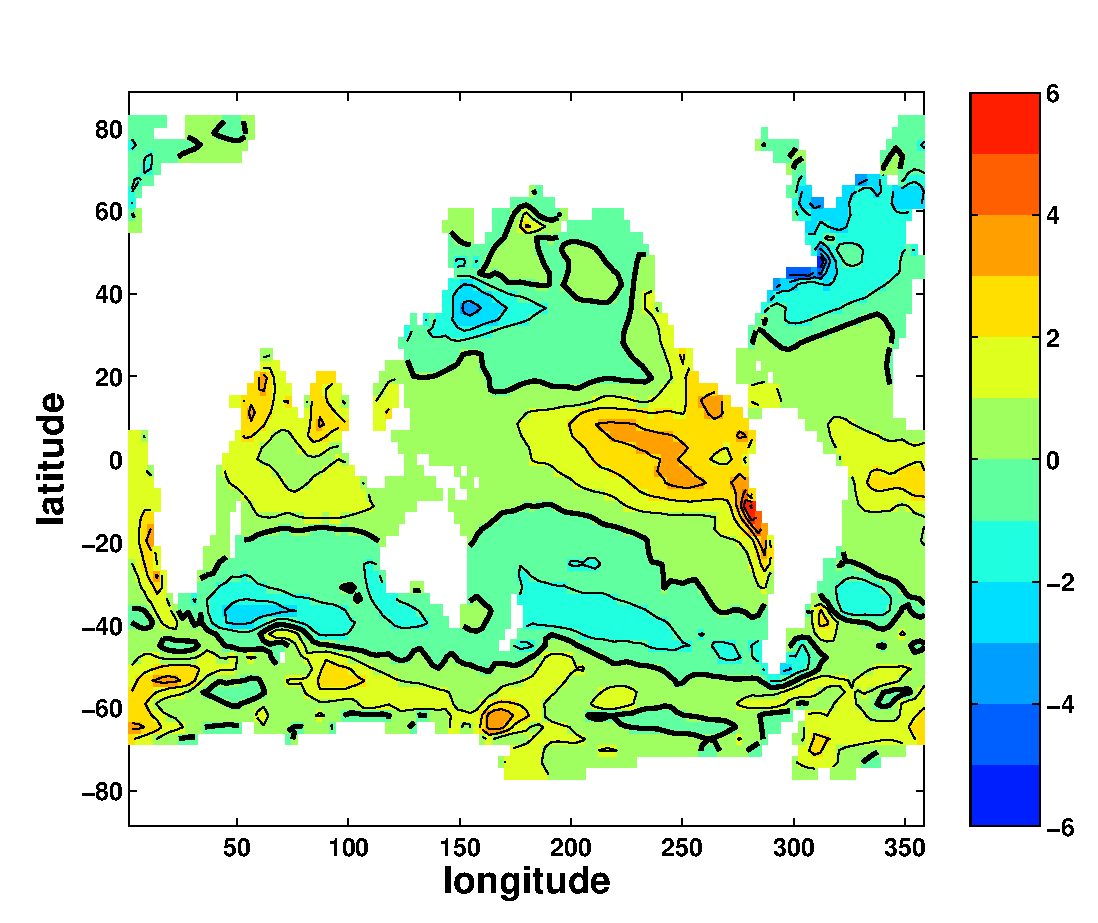
\includegraphics[width=\textwidth,height=.3\textheight]{part3/case_studies/biogeochem_tutorial/co2flux.eps}
\caption{Modelled annual  mean air-sea CO$_2$ flux (mol C m$^{-2}$ y$^{-1}$)
for pre-industrial steady-state. Positive indicates  flux of CO$_2$
from ocean to the atmosphere (out-gassing),
contour interval is 1 mol C m$^{-2}$ y$^{-1}$.}
\label{lFcarflux}
\end{center}
\end{figure}


\subsection{Equations Solved}

The physical ocean model velocity and diffusivities are used to
redistribute the 5 tracers within the ocean. Additional redistribution
comes from chemical and biological sources and sinks.  For any tracer
$A$:
\begin{equation}
  \frac{\partial A}{\partial t}=-\nabla \cdot (\vec{u^{*}} A)+\nabla \cdot
  (\mathbf{K}\nabla A)+S_A \nonumber \label{lEtrac}
\end{equation}
where $\vec{u^{*}}$ is the transformed Eulerian mean circulation
(which includes Eulerian and eddy-induced advection), $\mathbf{K}$ is
the mixing tensor, and $S_A$ are the sources and sinks due to
biological and chemical processes.

The sources and sinks are:
\begin{eqnarray}
S_{DIC} & = &  F_{CO_2} + V_{CO_2} + r_{C:P} S_{PO_4}  + J_{Ca} \label{lEsdic} \\
S_{ALK} & = &  V_{ALK}-r_{N:P} S_{PO_4}  + 2 J_{Ca} \label{lEsalk} \\
S_{PO_4}& = &  -f_{DOP} J_{prod} - \frac{\partial F_P}{\partial z} + \kappa_{remin} [DOP]\\
S_{DOP} & = &  f_{DOP} J_{prod} -\kappa_{remin} [DOP] \\
S_{O_2} & = & \left\{ \begin{array}{ll}
               -r_{O:P} S_{PO_4} & \mbox{if $O_2>O_{2crit}$} \\
                0  & \mbox{if $O_2<O_{2crit}$}
                      \end{array}
              \right. 
\end{eqnarray}
where:
\begin{itemize}
\item $F_{CO_2}$ is the flux of CO$_2$ from the ocean to the
  atmosphere
\item $V_{CO_2}$ is ``virtual flux'' due to changes in $DIC$ due to
  the surface freshwater fluxes
\item $r_{C:P}$ is Redfield ratio of carbon to phosphorus
\item $J_{Ca}$ includes carbon removed from surface due to calcium
  carbonate formation and subsequent cumulation of the downward flux
  of CaCO$_3$
\item $V_{ALK}$ is ``virtual flux'' due to changes in alkalinity due
  to the surface freshwater fluxes
\item $r_{N:P}$ Redfield ratio is nitrogen to phosphorus
\item $f_{DOP}$ is fraction of productivity that remains suspended in
  the water column as dissolved organic phosphorus
\item $J_{prod}$ is the net community productivity
\item $\frac{\partial F_P}{\partial z}$ is the accumulation of
  remineralized phosphorus with depth
\item $\kappa_{remin}$ is rate with which $DOP$ remineralizes back to
  $PO_4$
\item $F_{O_2}$ is air-sea flux of oxygen
\item $r_{O:P}$ is Redfield ratio of oxygen to phosphorus
\item $O_{2crit}$ is a critical level below which oxygen consumption
  if halted
\end{itemize}

These terms (for the first four tracers) are described more in
\cite{Dutkiewicz_etal_05} and by \cite{McKinley_etal_04} for the terms
relating to oxygen.


\subsection{Code configuration}

The model configuration for this experiment resides in
verification/dic\_example. The modifications to the code (in {\it
  verification/dic\_example/code}) are:
\begin{itemize}
\item{{\bf SIZE.h}: which dictates the size of the model domain
    (128x64x15).}
\item{\bf PTRACERS\_SIZE.h}: which dictates how many tracers to assign
  how many tracers will be used (5).
\item{\bf GCHEM\_OPTIONS.h}: provides some compiler time options for
  the {\it /pkg/gchem}. In particular this example requires that {\it
    DIC\_BIOTIC} and {\it GCHEM\_SEPARATE\_FORCING} be defined.
\item{\bf GMREDI\_OPTIONS.h}: assigns the Gent-McWilliam eddy
  parameterization options.
\item{\bf DIAGNOSTICS\_SIZE.h}: assigns size information for the
  diagnostics package.
\item{\bf packages.conf}: which dictates which packages will be
  compiled in this version of the model - among the many that are used
  for the physical part of the model, this also includes {\it
    ptracers}, {\it gchem}, and {\it dic} which allow the
  biogeochemical part of this setup to function.
\end{itemize}

\vspace{1cm}
\noindent
The input fields needed for this run (in {\it
  verification/dic\_example/input}) are:
\begin{itemize}
\item {\bf data}: specifies the main parameters for the experiment,
  some parameters that may be useful to know: {\it nTimeSteps} number
  timesteps model will run, change to 720 to run for a year {\it
    taveFreq} frequency with which time averages are done, change to
  31104000 for annual averages.
\item {\bf data.diagnostics}: species details of diagnostic pkg output
\item {\bf data.gchem}: specifics files and other details needed in
  the biogeochemistry model run
\item {\bf data.gmredi}: species details for the GM parameterization
\item {\bf data.mnc}: specifies details for types of output, netcdf or
  binary
\item {\bf data.pkg}: set true or false for various packages to be
  used
\item {\bf data.ptracers}: details of the tracers to be used,
  including makes, diffusivity information and (if needed) initial
  files. Of particular importance is the {\it PTRACERS\_numInUse}
  which states how many tracers are used, and {\it PTRACERS\_Iter0}
  which states at which timestep the biogeochemistry model tracers
  were initialized.
\item {\bf depth\_g77.bin}: bathymetry data file
\item {\bf eedata}: This file uses standard default values and does
  not contain customizations for this experiment.
\item {\bf fice.bin}: ice data file, needed for the biogeochemistry
\item {\bf lev\_monthly\_salt.bin}: SSS values which model relaxes
  toward
\item {\bf lev\_monthly\_temp.bin}: SST values which model relaxes
  toward
\item {\bf pickup.0004248000.data}: variable and tendency values need
  to restart the physical part of the model
\item {\bf pickup\_cd.0004248000.data}: variable and tendency values
  need to restart the cd pkg
\item {\bf pickup\_ptracers.0004248000.data}: variable and tendency
  values need to restart the the biogeochemistry part of the model
\item {\bf POLY3.COEFFS}: coefficient for the non-linear equation of
  state
\item {\bf shi\_empmr\_year.bin}: freshwater forcing data file
\item {\bf shi\_qnet.bin}: heat flux forcing data file
\item {\bf sillev1.bin}: silica data file, need for the
  biogeochemistry
\item {\bf tren\_speed.bin}: wind speed data file, needed for the
  biogeochemistry
\item {\bf tren\_taux.bin}: meridional wind stress data file
\item {\bf tren\_tauy.bin}: zonal wind stress data file
\end{itemize}


\subsection{Running the example}

You will first need to download the MITgcm code. Instructions for
downloading the code can be found in section 3.2.

\begin{enumerate}
\item{go to the build directory in verification/dic\_example:\\
    \hspace{1cm} $>$ {\it cd verification/dic\_example/build}}
\item{create the Makefile:\\
    \hspace{1cm} $>$ {\it ../../../tools/genmake2 -mods=code}}
\item{create all the links:\\
    \hspace{1cm} $>$ {\it make depend}}
\item{compile (the executable will be called mitgcmuv):\\
    \hspace{1cm} $>$ {\it make}}
\item{move the executable to the directory with all the inputs:\\
    \hspace{1cm} $>$ {\it mv mitgcmuv ../input/}}
\item{go to the input directory and run the model:\\
    \hspace{1cm} $>$ {\it cd ../input}\\
    \hspace{1cm} $>$ {\it ./mitgcmuv}}
\end{enumerate}
As the model is set up to run in the verification experiment, it only
runs for 4 timestep (2 days) and outputs data at the end of this short
run. For a more informative run, you will need to run longer. As set
up, this model starts from a pre-spun up state and initializes
physical fields and the biogeochemical tracers from the {\it pickup}
files.

Physical data (e.g. S,T, velocities etc) will be output as for any
regular ocean run. The biogeochemical output are:
\begin{itemize}
\item tracer snap shots: either netcdf, or older-style binary
  (depending on how {\it data.mnc} is set up). Look in {\it
    data.ptracers} to see which number matches which type of tracer
  (e.g. ptracer01 is DIC).
\item tracer time averages: either netcdf, or older-style binary
  (depending on how {\it data.mnc} is set up)
\item specific DIC diagnostics: these are averaged over {\it taveFreq}
  (set in {\it data}) and are specific to the dic package, and
  currently are only available in binary format:
  \begin{itemize}
  \item{\bf DIC\_Biotave}: 3-D biological community productivity (mol
    P m$^{-3}$ s$^{-1}$)
  \item{\bf DIC\_Cartave}: 3-D tendencies due to calcium carbonate
    cycle (mol C m$^{-3}$ s$^{-1}$)
  \item{\bf DIC\_fluxCO2ave}: 2-D air-sea flux of CO$_2$ (mol C
    m$^{-2}$ s$^{-1}$)
  \item{\bf DIC\_pCO2tave}: 2-D partial pressure of CO$_2$ in surface
    layer
  \item{\bf DIC\_pHtave}: 2-D pH in surface layer
  \item{\bf DIC\_SurOtave}: 2-D tendency due to air-sea flux of O$_2$
    (mol O m$^{-3}$ s$^{-1}$)
  \item{\bf DIC\_Surtave}: 2-D surface tendency of DIC due to air-sea
    flux and virtual flux (mol C m$^{-3}$ s$^{-1}$)
  \end{itemize}
\end{itemize}


%% \subsection{Reference Material}

%% \Hpar
%% Dutkiewicz. S., A. Sokolov, J.Scott and P. Stone, 2005:
%% A Three-Dimensional Ocean-Seaice-Carbon Cycle Model and its Coupling
%% to a Two-Dimensional Atmospheric Model: Uses in Climate Change Studies,
%% Report 122, Joint Program of the Science and Policy of Global Change,
%% M.I.T., Cambridge, MA.\\
%% (http://web.mit.edu/globalchange/www/MITJPSPGC\_Rpt122.pdf)
%% \Hpar
%% Follows, M., T. Ito and S. Dutkiewicz, 2005:
%% A Compact and Accurate Carbonate Chemistry Solver for Ocean
%% Biogeochemistry Models. {\it Ocean Modeling}, in press.
%% \Hpar
%% Gent, P. and J. McWilliams, 1990:
%% Isopycnal mixing in ocean circulation models.
%% {\it Journal of Physical Oceanography}, 20, 150 -- 155.
%% \Hpar
%% Jiang, S., P.H. Stone, and P. Malanotte-Rizzoli,
%% An assessment of the Geophysical Fluid Dynamics Laboratory
%% ocean model with coarse resolution: Annual-mean climatology,
%% {\it Journal of Geophysical Research}, 104, 25623 -- 25645, 1999.
%% \Hpar
%% Levitus, S. and T.P. Boyer, 1994:
%% {\it World Ocean Atlas 1994 Volume 4: Temperature},
%% NOAA Atlas NESDIS 4, U.S. Department of Commerce,
%% Washington, D.C., 117pp.
%% \Hpar
%% Levitus, S., R. Burgett, and T.P. Boyer, 1994:
%% {\it World Ocean Atlas 1994 Volume 3: Salinity},
%% NOAA Atlas NESDIS 3, U.S. Department of Commerce,
%% Washington, D.C., 99pp.
%% \Hpar
%% McKinley, G., M.J. Follows and J.C. Marshall, 2004:
%% Mechanisms of air-sea CO$_2$ flux variability in the Equatorial Pacific
%% and the North Atlantic.
%% {\it Global Biogeochemical Cycles}, 18, doi:10.1029/2003GB002179.
%% \Hpar
%% Trenberth, K., J. Olson, and W. Large, 1989:
%% {\it A global wind stress climatology based on ECMWF analyses,
%% Tech. Rep. NCAR/TN-338+STR},
%% National Center for Atmospheric Research, Boulder, Colorado.
%% \Hpar
%% Wanninkhof, R., 1992:
%% Relationship between wind speed and gas exchange over the ocean,
%% {\it Journal of Geophysical Research}, 97, 7373 -- 7382.

